\section*{6.17}
%\addcontentsline{toc}{section}{Question 1}

a) On pose les conditions suivantes selon le problème :
\begin{gather*}
    e(t) = 2\delta(t-1),\ L = 2,\ R = 50,\ C = 0.005,\ v_c(0)=10,\ v_c'(0)=0 \\
    LC = 0.01,\ RC = 0.25
\end{gather*}

L'ÉDO à résoudre est :
\begin{align*}
    0.01v_c'' + 0.25v_c' + v_c = 2\delta(t-1)
\end{align*}

En utilisant la fonction ets\textunderscore specfunc\textbackslash solved sur la Ti
sur l'ÉDO précédente, on trouve :
\begin{gather*}
    \specfunc \prt{0.01\cdot\dv{^2}{t^2}y(t) + 0.25\cdot\dv{}{t}y(t) + y(t)
    = 2\delta(t-1),\{y(t),10,0\}} \\
    \implies v_c(t) = \f{40}{3}\prt{e^{5-5t}-e^{20-20t}}u(t-1)
    +\f{10}{3}\prt{4 e^{-5t}-e^{-20t}}u(t)
\end{gather*}

b) Voici le graphique de la tension :
\begin{center}
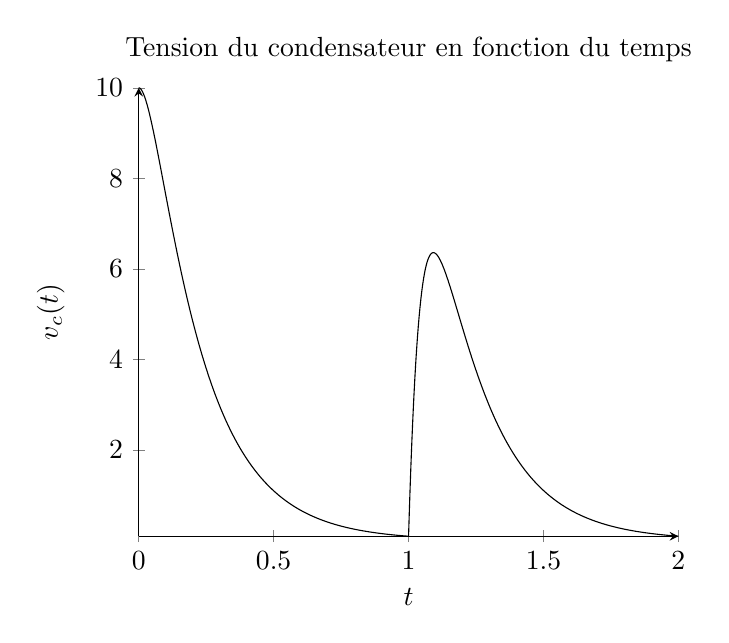
\begin{tikzpicture}
\begin{axis}[
    title = Tension du condensateur en fonction du temps,
    extra y ticks       = 0,
    extra y tick labels = ,
    extra y tick style  = { grid = major },
    axis lines = left,
    xlabel = \(t\),
    ylabel = {\(v_c(t)\)},
]
% Plot de la tension
\addplot [
    domain=0:1, 
    samples=500, 
    color=black,
    ] {(10/3)*(4*e^(-5*x) -e^(-20*x))};

\addplot [
    domain=1:2, 
    samples=500, 
    color=black,
    ] {(10/3)*(4*e^(-5*x) -e^(-20*x)) + (40/3)*(e^(5-5*x)-e^(20-20*x))};
\end{axis}
\end{tikzpicture}
\end{center}
